\documentclass[10pt]{beamer}
\usepackage{ragged2e} % \justifying
\usetheme{metropolis}           % Use metropolis theme
\title{Vision-based Autonomous Landing in Catastrophe-Struck Environments}
\subtitle{\textit{Authors:} Mayank Mittal, Abhinav Valada, Wofram Burgard}
\date{\today}
\author{Michele Cipriano}
\institute{Control Problems in Robotics: Modeling and control of
    multi-rotor UAVs\\Department of Computer, Control and Management
    Engineering\\Sapienza University of Rome}

% Fontsize of figure smaller than normalsize:
\setbeamerfont{caption}{size=\scriptsize}

\begin{document}
\nocite{*}

    \maketitle

    \begin{frame}{Introduction}
        \begin{columns}[c,onlytextwidth]
            \column{0.5\textwidth}
                \vspace*{\fill}
                Intro.
                \begin{itemize}
                    \item Why it's important (bioradiolocation, also emergency landing)
                    \item previous work
                \end{itemize}
                \vspace*{\fill}

            \column{0.5\textwidth}
                \begin{figure}
                    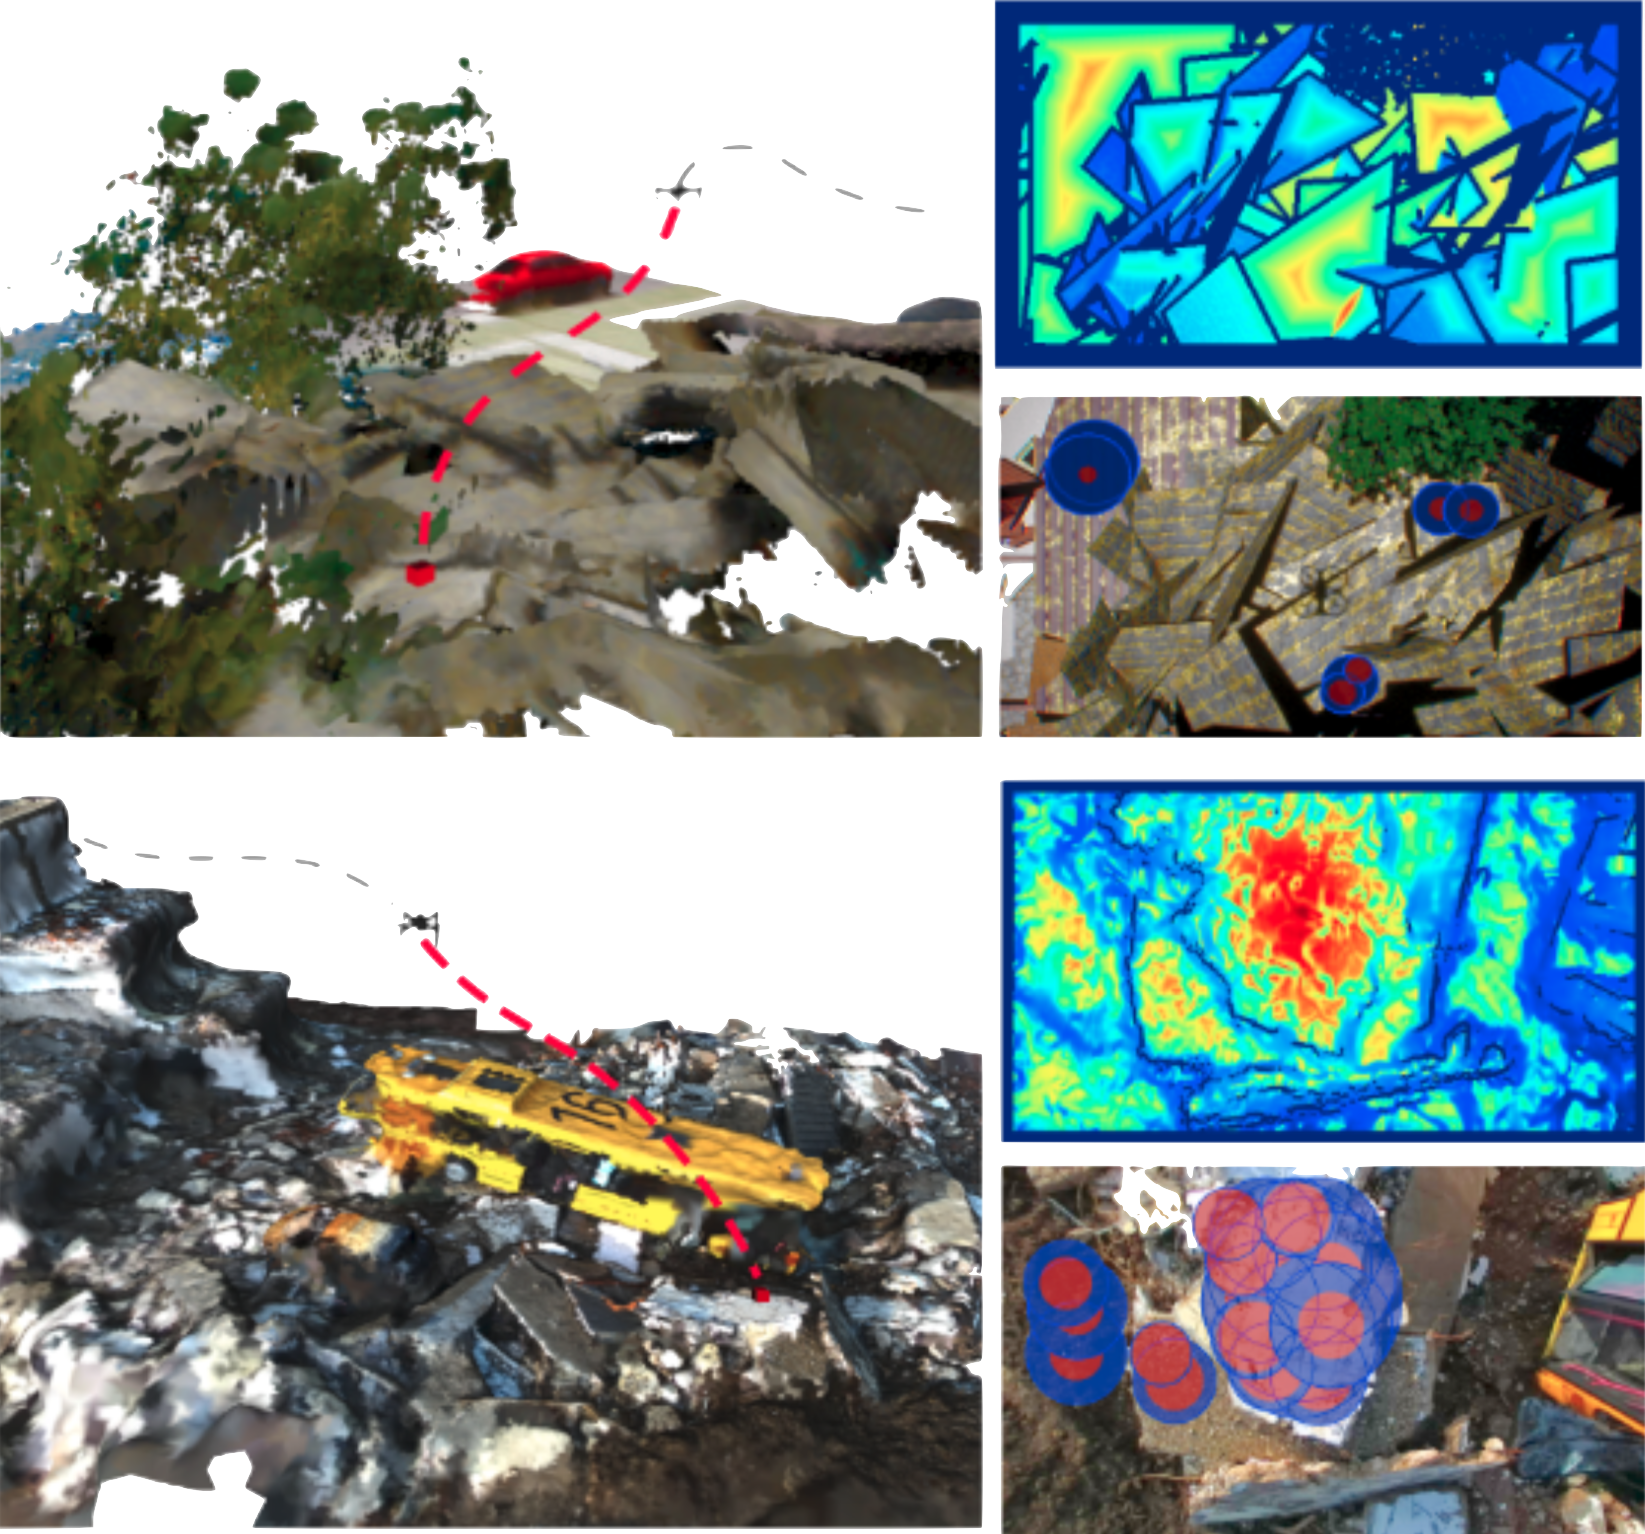
\includegraphics[width=\textwidth]{images/Fig1.png}
                \end{figure}
        \end{columns}
    \end{frame}

    \begin{frame}{Technical Approach}
        Brief introduction to ch. 3, describe approach and then discuss details.
        \begin{itemize}
            \item State Estimation
            \item Landing Site Detection
            \item 3D Volumetric Mapping
            \item Landing Trajectory Estimation
        \end{itemize}
    \end{frame}

    \begin{frame}{Technical Approach: State Estimation}
        \justifying
        \begin{itemize}
            \item downward-facing stereo camera
            \item \textbf{ORB-SLAM2} (oriented FAST and rotated BRIEF)
            \item multi-sensor fusion (EKF) using IMU, barometer and GPS
            \item sensor precalibrated with Kalibr toolbox
        \end{itemize}
    \end{frame}

    \begin{frame}{Technical Approach: Landing Site Detection}
        \justifying
        Confidence in \textbf{\textsc{Depth Information}} $J_{DE}$:
        \begin{equation*}
            J_{DE}(p) = 1 - \frac{D(p)^2 - min\{D^2\}}{max\{D^2\}}
        \end{equation*}
        with $D$ depthmap obtained from the stereo camera and $p=(x,y)$
        pixel in the depthmap.
    \end{frame}

    \begin{frame}{Technical Approach: Landing Site Detection}
        \justifying
        \textbf{\textsc{Flatness Information}} $J_{FL}$:
        \begin{gather*}
            di(B, p) = min\Big\{\|p-q\| \Big| B(q)=1\Big\} \\
            J_{FL}(p) = di(Canny(D), p)
        \end{gather*}
        with $B$ binary image and $p, q$ pixels in the image plane. $Canny$
        applies the Canny edge detector over the depthmap $D$.
    \end{frame}

    \begin{frame}{Technical Approach: Landing Site Detection}
        \justifying
        \textbf{\textsc{Steepness Information}} $J_{N}$:
        \begin{itemize}
            \item point cloud from the depthmap in global frame
            \item average 3D gradients algorithm to estimate normals map $N$
            \item evaluate deviation of the normalized surface normal
                $\hat{n}$ wrt z-axis $\hat{z}$ in the world frame:
                $\theta = cos^{-1}(\hat{n}^T\hat{z})$
            \item compute $n(p)$ steepness score for each pixel $p$ given
                $\theta_{th}=\pi/12$ maximum tolerable slope
        \end{itemize}
        \begin{equation*}
            n(p) = exp\left\{ -\frac{\theta^2}{2\theta^2_{th}} \right\}
        \end{equation*}
    \end{frame}

    \begin{frame}{Technical Approach: Landing Site Detection}
        \justifying
        \textbf{\textsc{Energy Consumption Information}} $J_{EC}$:
        \begin{equation*}
            J_{EC}(p) = \int_{t_0}^{t_f} P(t)dt
        \end{equation*}
        with $t_0$ and $t_f$ time of flight to reach $p$ and $P(t)$
        instantaneous battery power. Approximate the integral with Euclidean
        distance between the UAV and $p$.
    \end{frame}

    \begin{frame}{Technical Approach: Landing Site Detection}
        \justifying
        Scale the costmaps to the same range through min-max normalization
        and compute the final decision map $J$ taking a weighted sum:
        \begin{gather*}
            J = c_1 J_{DE} + c_2 J_{FL} + c_3 J_{N} + c_4 J_{EC} \\
            c_i \in [0, 1] \quad \sum_i c_i = 1
        \end{gather*}
        \vspace{-0.5cm}
        \begin{itemize}
            \item keep the sites checking whether the UAV could actually land
            \item k-d tree to efficiently store new landing sites
            \item hierarchical clustering algorithm to agglomerate sites
        \end{itemize}
    \end{frame}

    \begin{frame}{Technical Approach: Landing Site Detection}
        \begin{figure}
            \caption{
                \justifying
                Overview of the landing site detection algorithm. In
                the costmaps, red indicates high score while blue indicates
                a lower score. Detected landing sites are projected onto
                a 3D reconstruction of the environment.}
            \vspace{-0.3cm}
            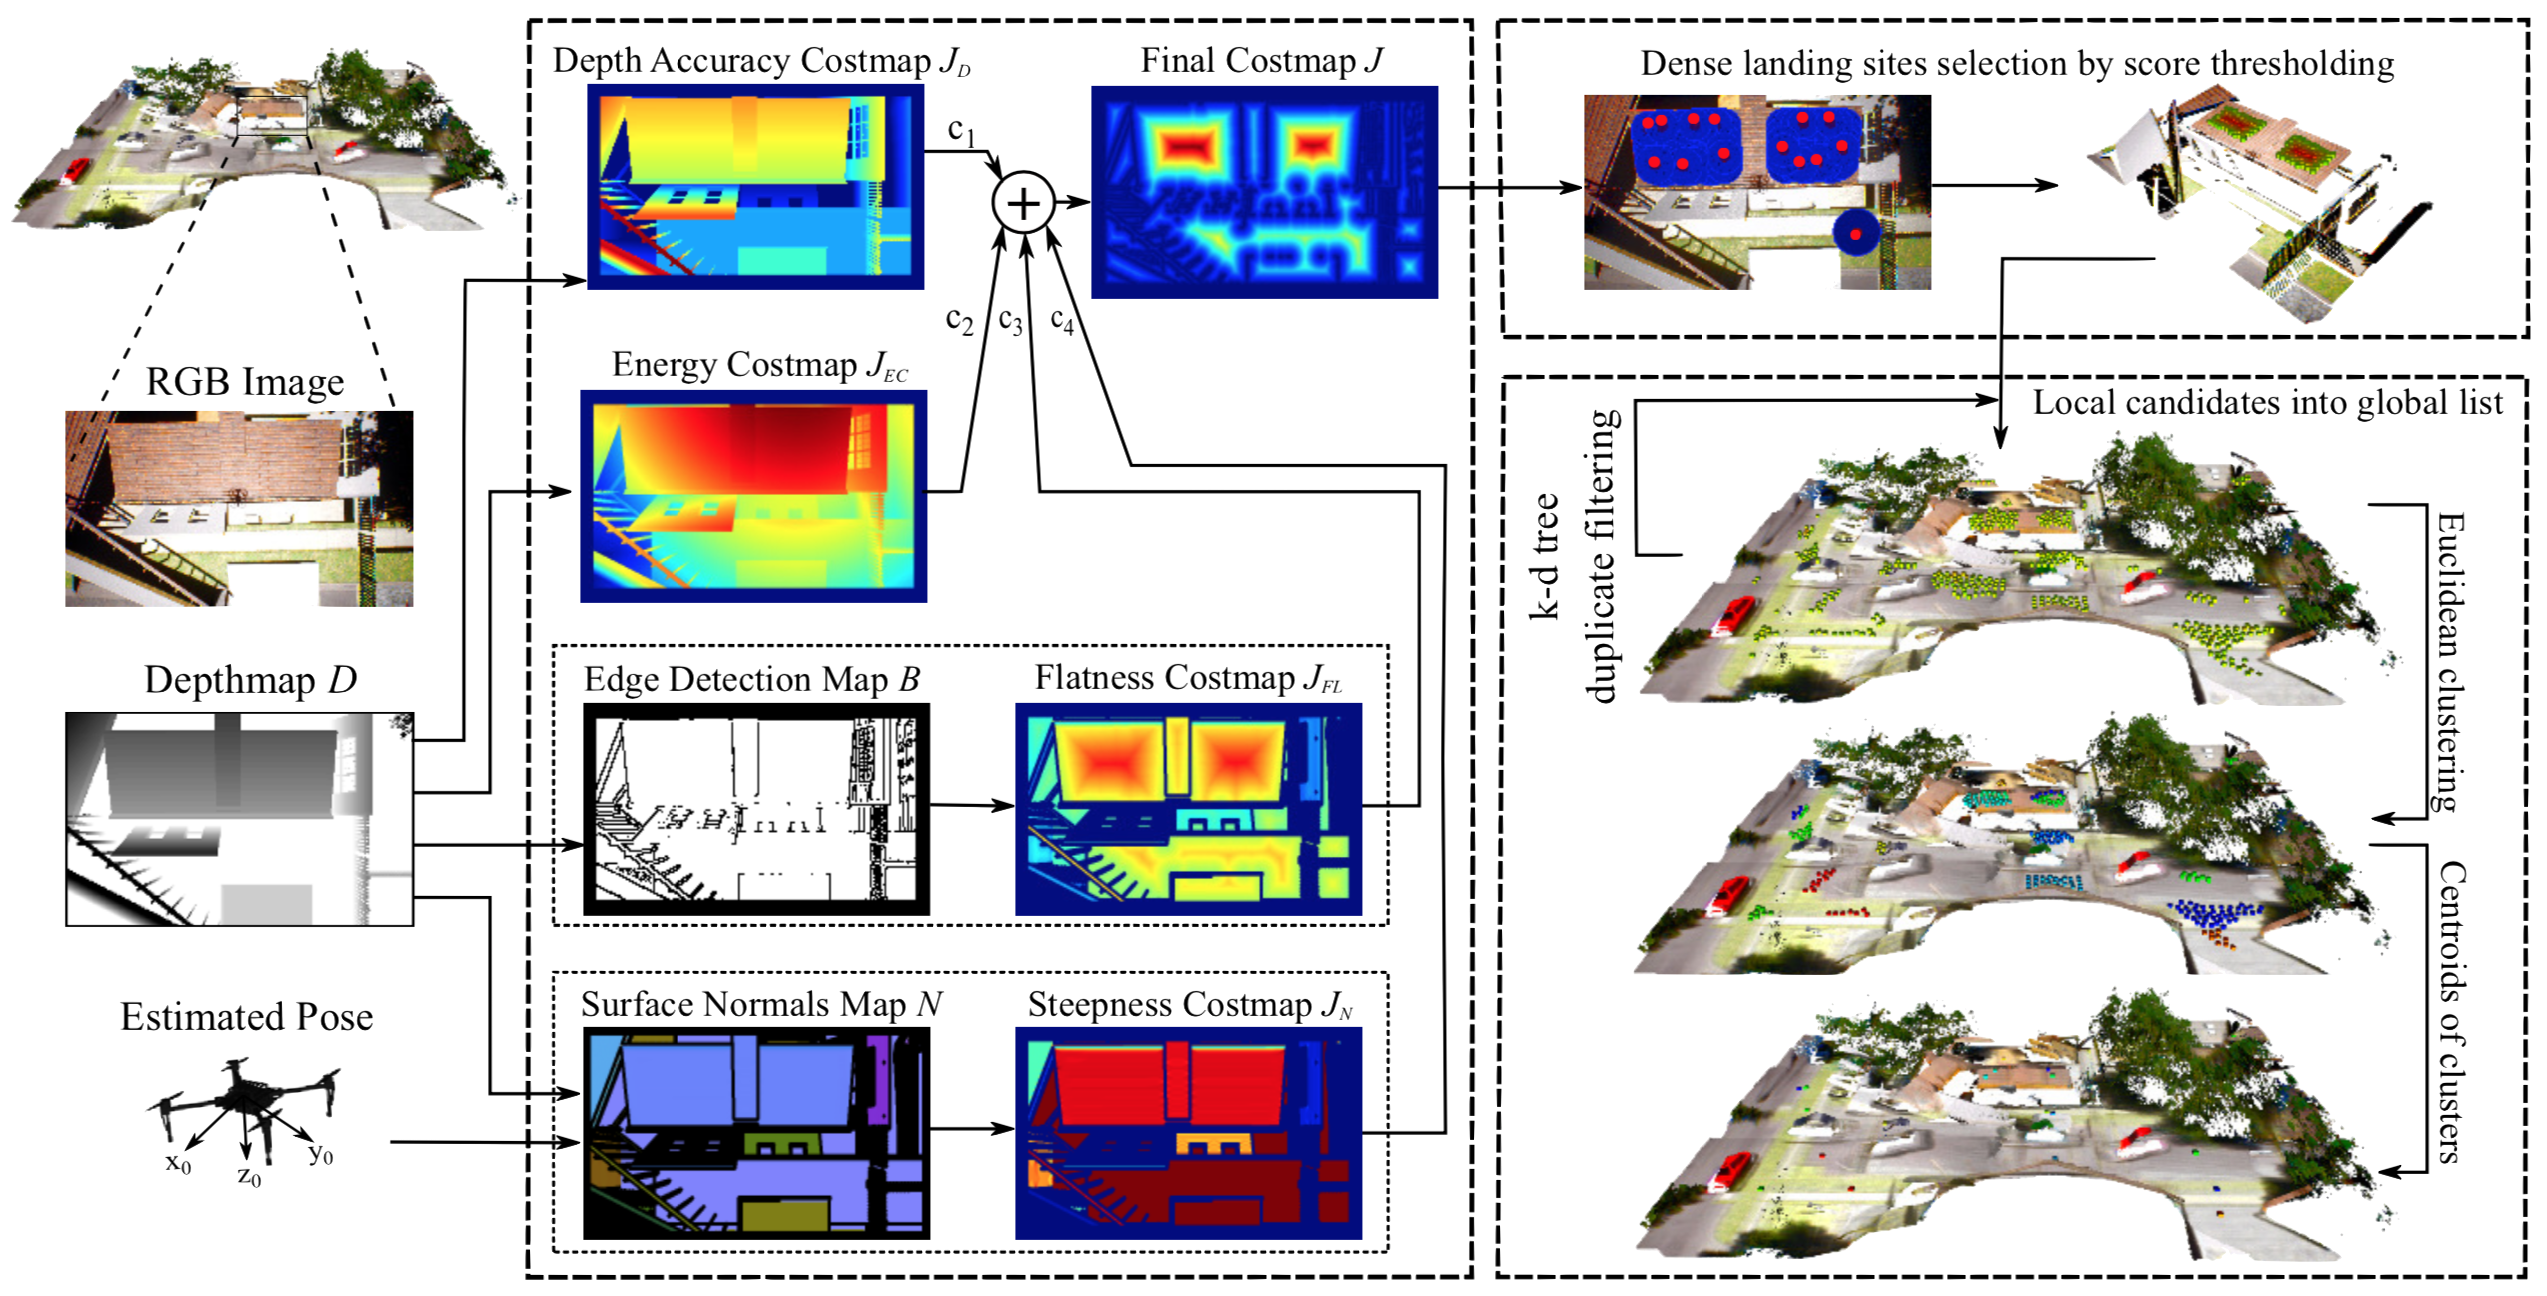
\includegraphics[width=\textwidth]{images/Fig3.png}
        \end{figure}
    \end{frame}

    \begin{frame}{Technical Approach: 3D Volumetric Mapping}
        Probabilistic volumetric map:
        \begin{itemize}
            \item navigation and planning
            \item low-resolution map ($0.5$m) using \textbf{OctoMaps}
            \item faster trajectory planning
        \end{itemize}

        3D textured mesh:
        \begin{itemize}
            \item dynamic map growing using \textbf{Voxblox}
            \item high-resolution mesh transmitted to the rescue team
        \end{itemize}
    \end{frame}

    \begin{frame}{Technical Approach: Landing Trajectory Estimation}
        Minimum-jerk trajectory generator with non-linear optimization:
        \begin{columns}[c,onlytextwidth]
            \column{0.5\textwidth}
                \justifying
                \begin{itemize}
                    \item \textbf{RRT*} for collision free path
                    \item line-of-sight for waypoints
                    \item minimum-snap polynomial trajectories using
                        differential flat model
                    \item high speed arcs in obstacles free regions
                    \item low velocities in tight places
                \end{itemize}
                %Guarantees high speed arcs in obstacles free regions and low
                %velocities in tight places.
            \column{0.5\textwidth}
                \begin{figure}
                    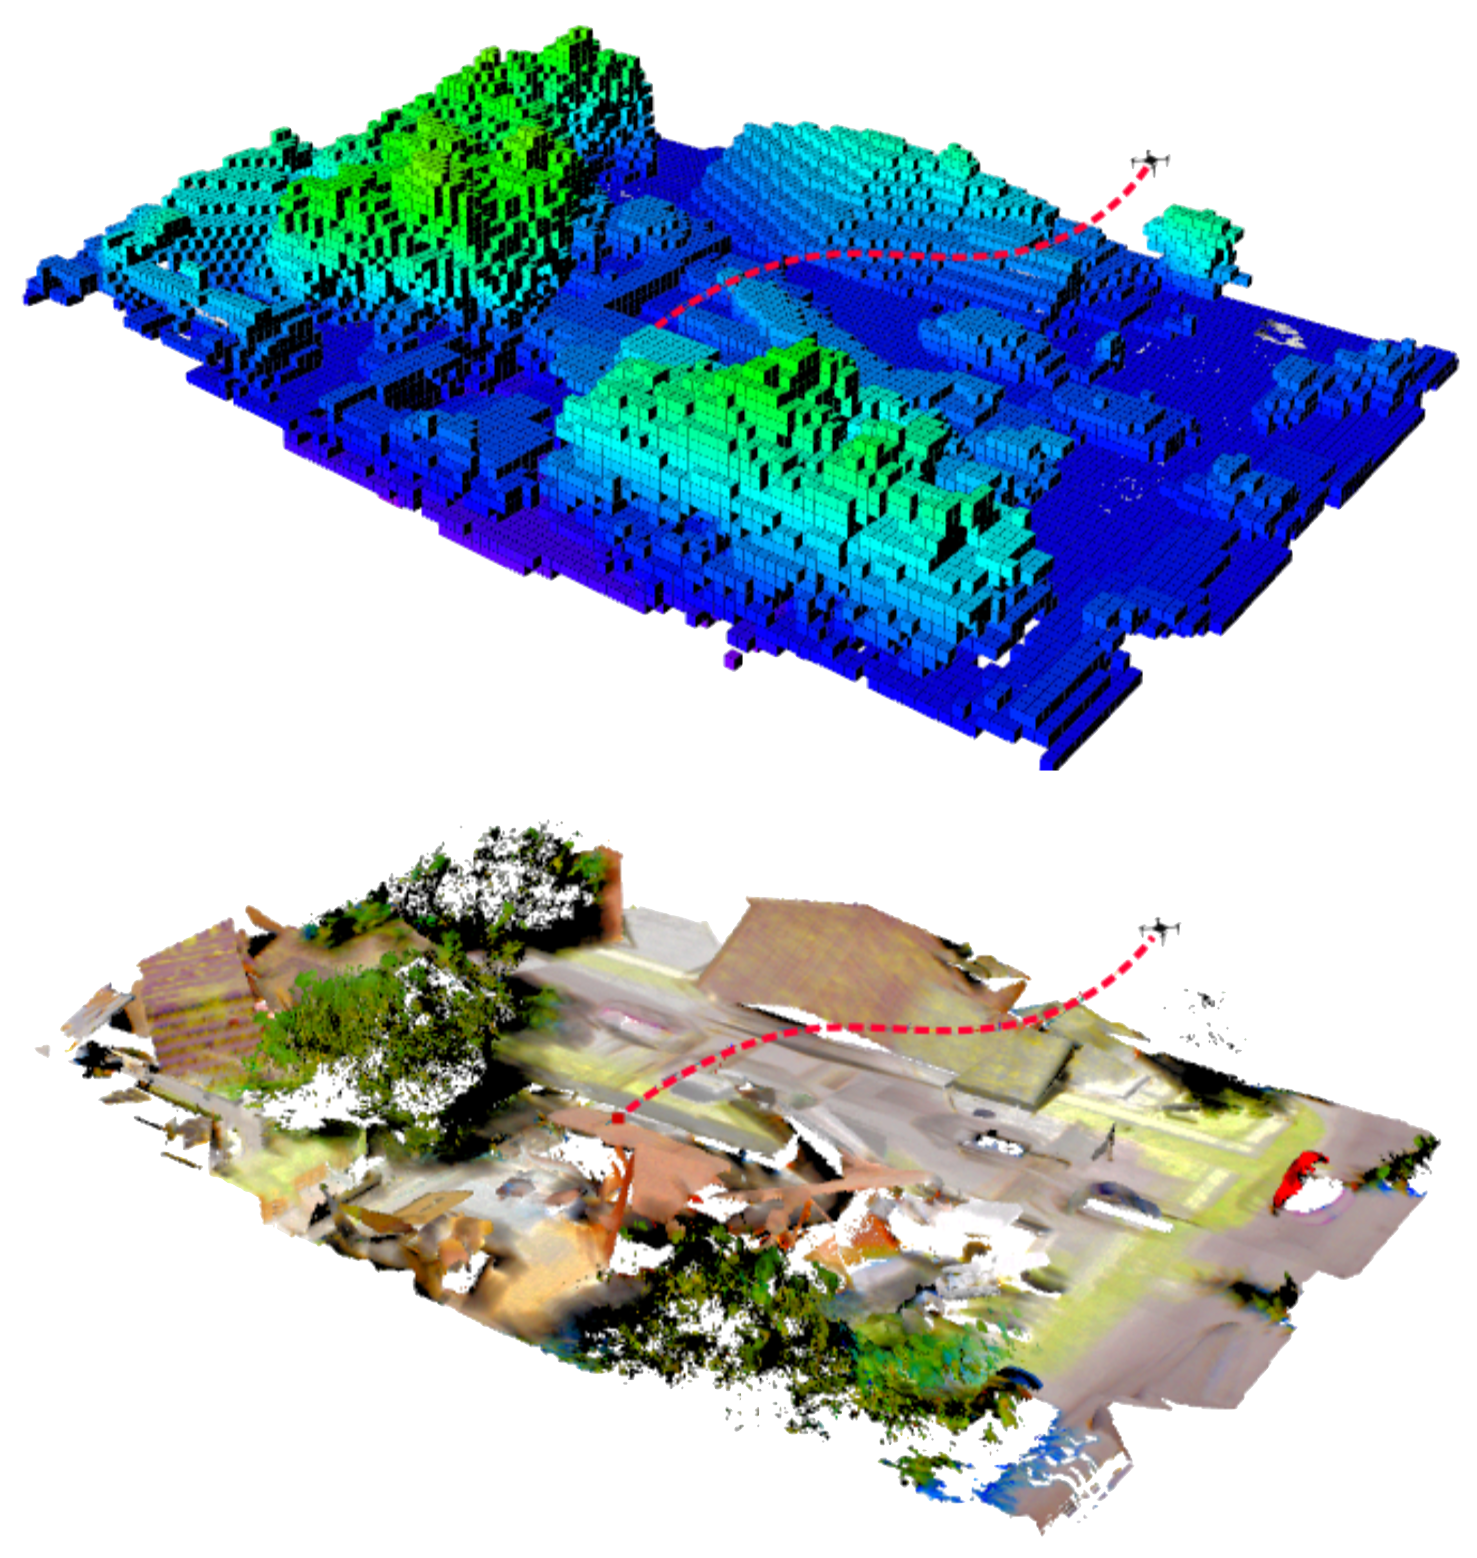
\includegraphics[width=\textwidth]{images/Fig4.png}
                \end{figure}
        \end{columns}
    \end{frame}

    \begin{frame}{Experimental Evaluation}
        Description:
        \begin{itemize}
            \item Hyperrealistic Simulation
            \item Real-World Outdoor (Training Center for Rescue, Germany)
        \end{itemize}
        + computation costs
    \end{frame}

    \begin{frame}{Experimental Evaluation: Hyperrealistic Simulation}
        Hyperrealistic Simulation Experiments
    \end{frame}

    \begin{frame}{Experimental Evaluation: Real-World Outdoor}
        Real-World Outdoor Experiments
    \end{frame}

    \begin{frame}{Experimental Evaluation: Computation Costs}
        \begin{columns}[c,onlytextwidth]
            \column{0.5\textwidth}
                Computation costs

            \column{0.5\textwidth}
                \vspace{0.4cm}
                \begin{figure}
                    \centering
                    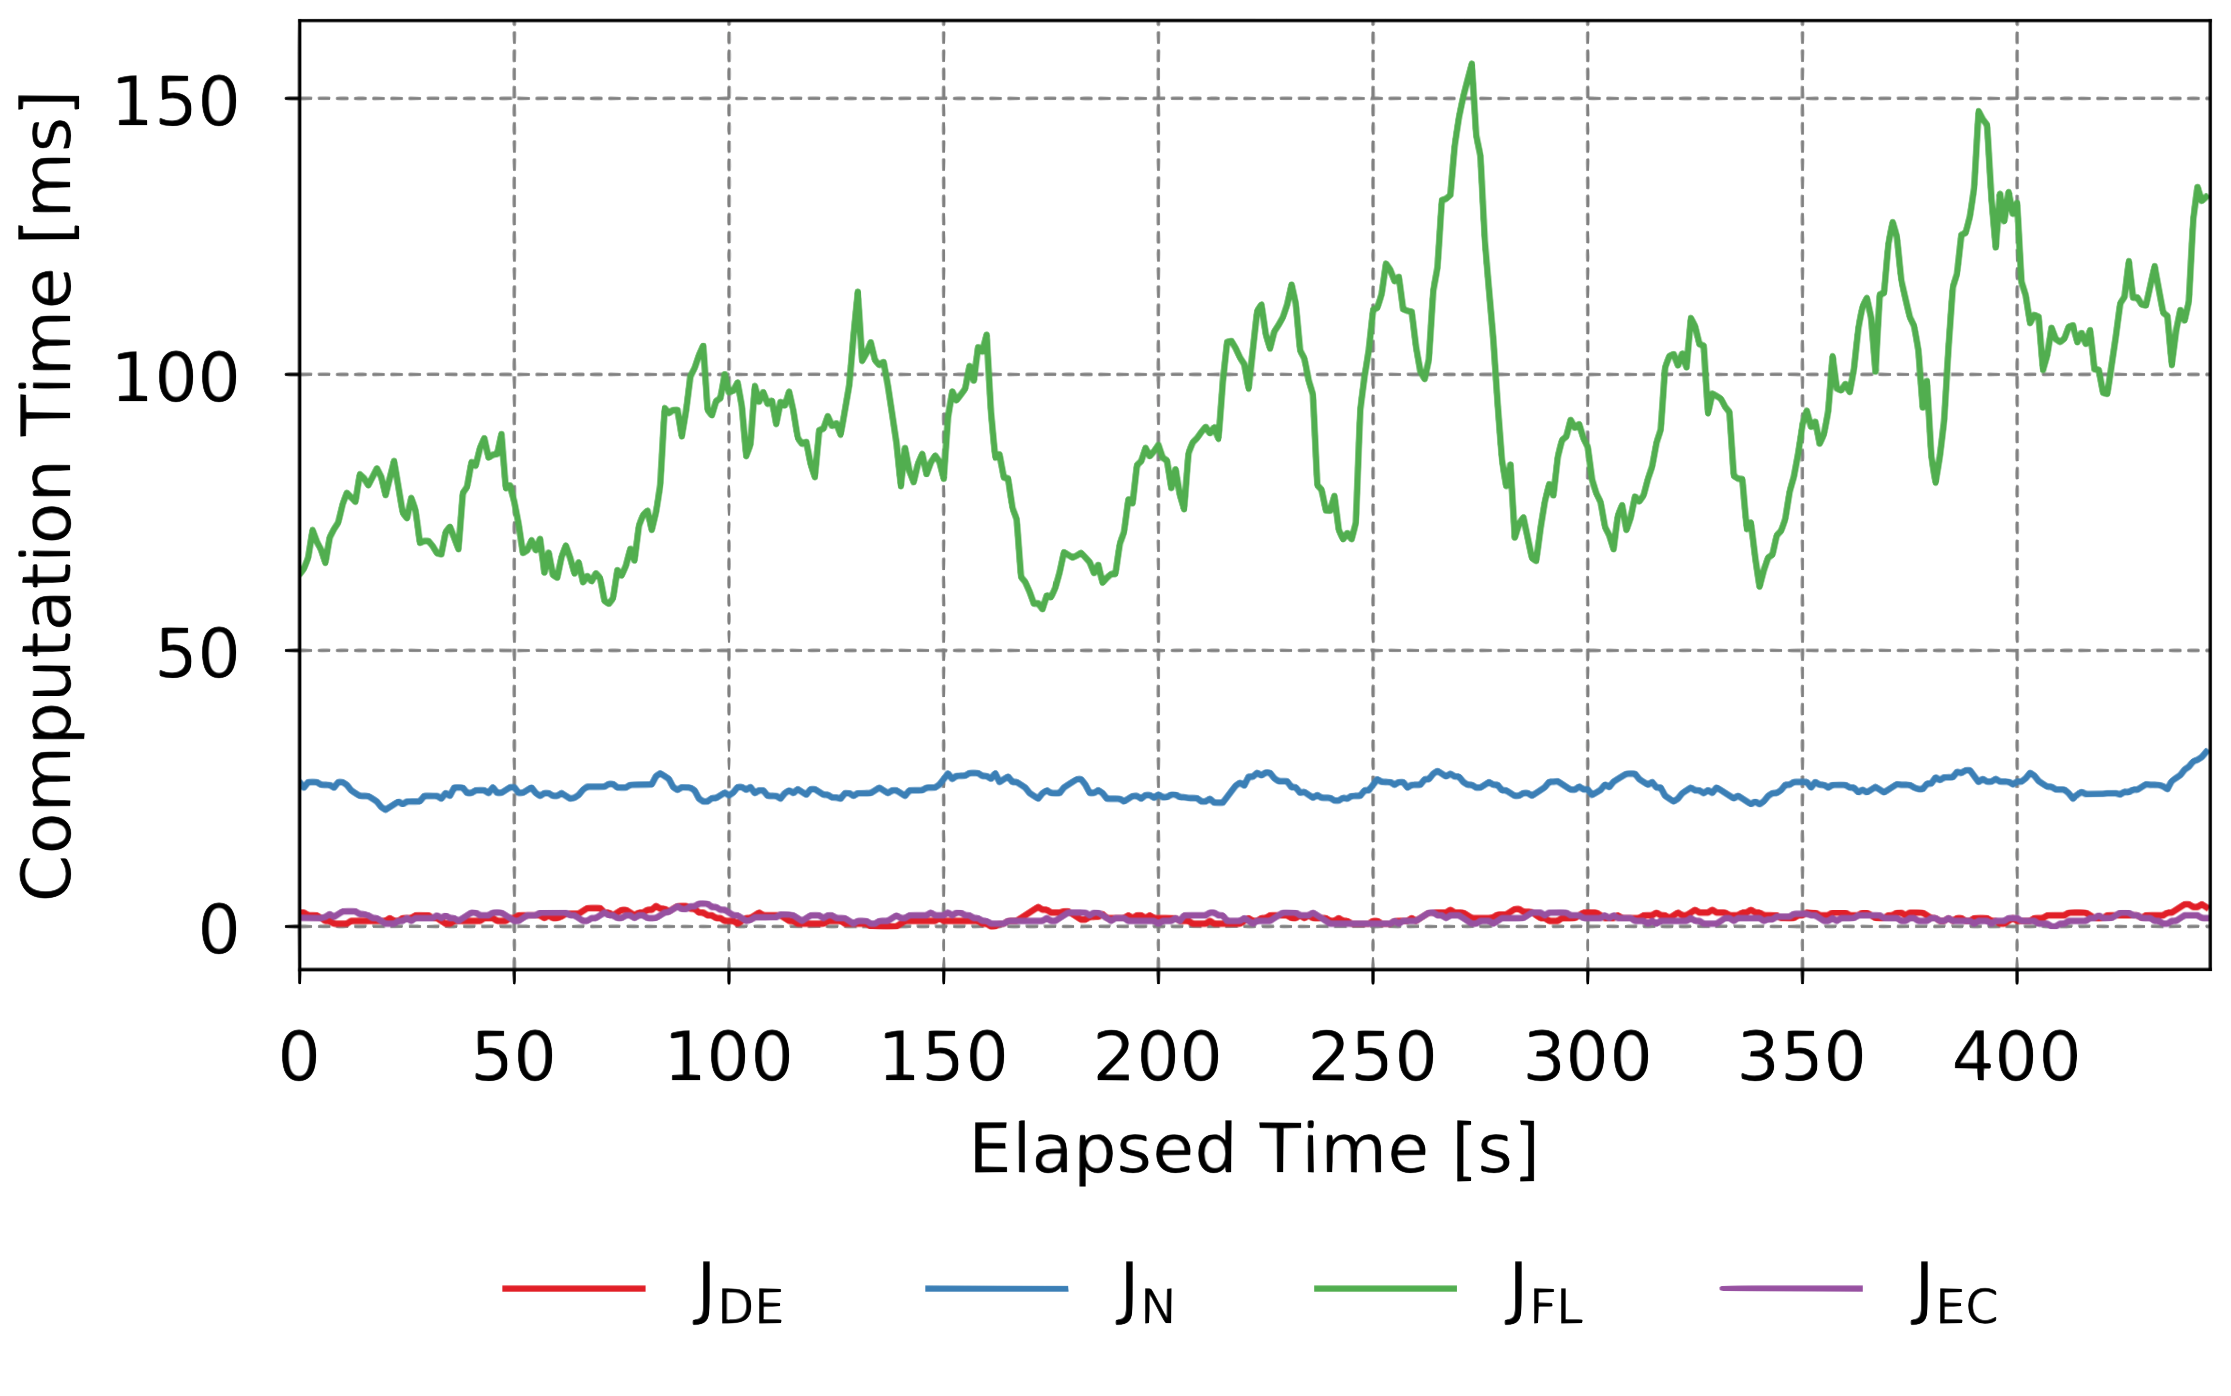
\includegraphics[width=\textwidth]{images/Fig8a.png}
                \end{figure}
                \vspace{-0.8cm}
                \begin{figure}
                    \centering
                    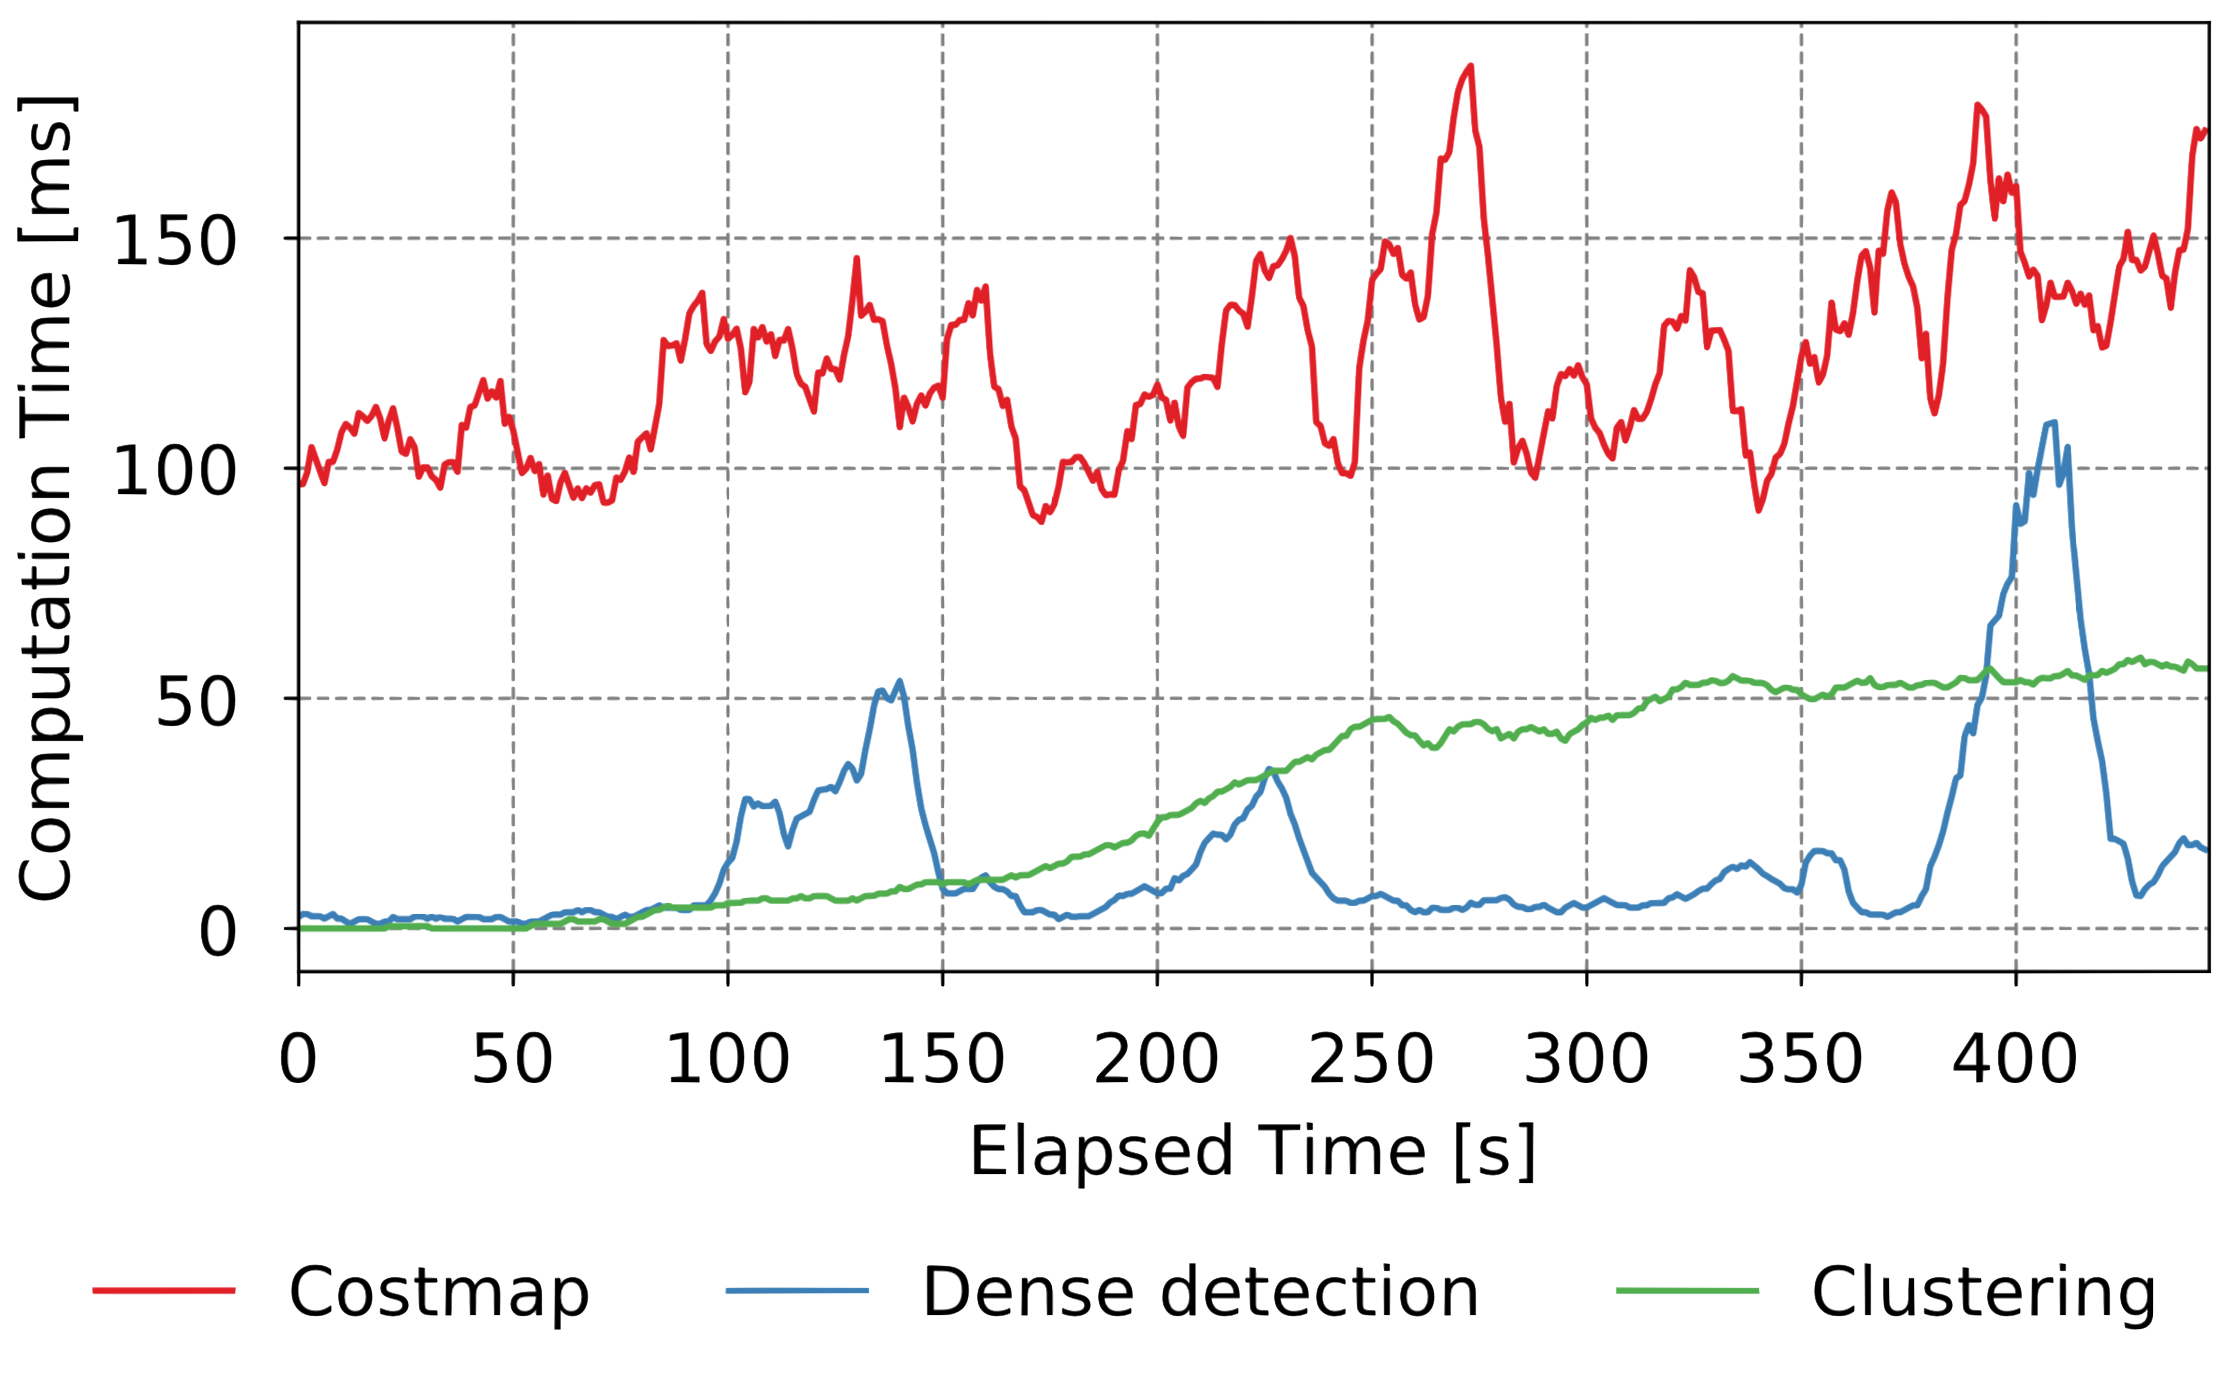
\includegraphics[width=\textwidth]{images/Fig8b.png}
                \end{figure}
        \end{columns}
    \end{frame}

    \begin{frame}{Conclusion}
        Conclusion.
    \end{frame}

    \begin{frame}[standout]
        Q\&A
    \end{frame}

    \appendix

    \begin{frame}{References}
        \bibliography{bibliography}
        \bibliographystyle{ieeetr}
    \end{frame}

\end{document}
